\chapter{Decidability}

\lecture{10}{2025-12-1}{}

\section{Decidability}

If we have a algorithm, we want to check if the problem is solvable or not on the computer. We need a TM to decide it, i.e. accept or reject in finite \# steps.

\begin{definition*}
    We first give some definitions of the languages.
    \begin{definition}[$A$]
        $A$ is the language \[
            A = \{ \langle M, w \rangle \mid M: \text{ TM that accepts } w \}
        \]
    \end{definition}
    \begin{definition}[$E$]
        $E$ is the language \[
            E = \{ \langle M \rangle \mid M: \text{ TM},\ L(M) = \emptyset \}
        \]
    \end{definition}
    \begin{definition}[$EQ$]
        $EQ$ is the language \[
            EQ = \{ \langle M_1, M_2 \rangle \mid M_1, M_2: \text{ TM},\ L(M_1) = L(M_2) \}
        \]
    \end{definition}
\end{definition*}

\newpage

\subsection{$A_{\text{DFA}}$ is Decidable}

\begin{eg}
    Consider the language \[
        A_{\text{DFA}} = \{ \langle B, w \rangle \mid B \text{ is a DFA that accepts } w \}
    \]
\end{eg}

The input of the problem is a pair of a DFA and a string, note that both can be encoded as a string.

\begin{idea}
    Input: $\langle B, w \rangle$ where $B$ is a DFA and $w$ is a string.
    \begin{enumerate}[label=$\arabic*^\circ$]
        \item Simulate $B$ on input $w$.
        \item If $B$ accepts, then accept. If $B$ rejects, then reject.
    \end{enumerate} 
\end{idea}

We first put \[
    B = (Q, \Sigma, \delta, q_0, F)
\]
into the tape, then we put $w$ after it. Then checking if $w \in \Sigma^*$. Then simulate $w$ according to $\delta$. After reading the whole $w$, check if the current state is in $F$.

\subsection{$A_{\text{NFA}}$ is Decidable}

\begin{eg}
    Consider the language \[
        A_{\text{NFA}} = \{ \langle B, w \rangle \mid B \text{ is an NFA that accepts } w \}
    \]
\end{eg}

We can use the subset construction to convert NFA to DFA, then use the previous algorithm.

\subsection{$A_{\text{REX}}$ is Decidable}

\begin{eg}
    Consider the language \[
        A_{\text{REX}} = \{ \langle R, w \rangle \mid R: \text{ regular expression generates } w \}
    \]
\end{eg}

We first convert $R$ to an NFA $B$ using the standard construction, then use the previous algorithm.

\begin{remark}
    We have a procedure to convert a regular expression to an equivalent NFA. Then we can use the algorithm for $A_{\text{NFA}}$ to decide $A_{\text{REX}}$.
\end{remark}

The key idea is that we have procedures to convert of regular languages is in \textbf{\red{finite}} steps.

\subsection{$E_{\text{DFA}}$ is Decidable}

\begin{eg}
    Consider the language \[
        E_{\text{DFA}} = \{ \langle A \rangle \mid A: \text{ DFA},\ L(A) = \emptyset \}
    \]
    i.e. $A$ accepts no strings.
\end{eg}

\begin{idea}
    Input: $\langle A \rangle$ where $A$ is a DFA.
    \[
        \text{DFA accepts something}\ \iff\ \text{reaching a final state from q0 after several links}
    \]
    \begin{enumerate}[label=$\arabic*^\circ$]
        \item Mark $q_0$.
        \item Repeat until no new state is marked:
        \begin{itemize}
            \item For each transition $\delta(q, a) = p$, if $q$ is marked, then mark $p$.
        \end{itemize}
        \item If no $q \in F$ is marked, then accept. Otherwise, reject.
    \end{enumerate}
\end{idea}

\vspace{1em}

There are at least one new $q \in Q$ marked in each iteration, so the algorithm halts in at most $|Q|$ iterations.

\subsection{$EQ_{\text{DFA}}$ is Decidable}

\begin{eg}
    Consider the language \[
        EQ_{\text{DFA}} = \{ \langle A, B \rangle \mid A, B: \text{ DFA},\ L(A) = L(B) \}
    \]
\end{eg}

\begin{idea}
    Let a DFA $C$ be the \textbf{exclusive or} of $A$ and $B$. \[
        L(A) = L(B) \iff L(C) = \emptyset
    \]
    \begin{figure}[H]
        \centering
        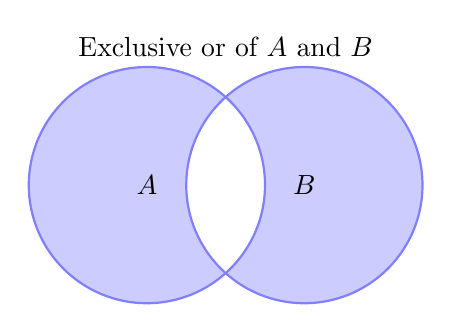
\begin{tikzpicture}
            [filled/.style={fill=blue!20, draw=blue!50, thick}, outline/.style={draw=blue!50, thick}]
            \draw[filled, even odd rule] (0,0) circle (1.5cm) node {$A$}
                                        (0:2cm) circle (1.5cm) node{$B$};
            \node[anchor=south] at (current bounding box.north) {Exclusive or of $A$ and $B$};
        \end{tikzpicture}
    \end{figure}
    Formally, we can construct $C$ as follows:
    \[
        L(C) = (L(A) \cap \overline{L(B)}) \cup (\overline{L(A)} \cap L(B))
    \]
    \begin{itemize}
        \item $B$ is DFA $\implies$ $\overline{B}$ is DFA.
        \item $A, B$ DFA $\implies$ $A \cap B$ is DFA.
    \end{itemize}
\end{idea}

\subsection{$A_{\text{CFG}}$ is Decidable}

\begin{eg}
    Consider the language \[
        A_{\text{CFG}} = \{ \langle G, w \rangle \mid G: \text{ CFG that generates } w \}
    \]
\end{eg}

\begin{note}
    The possible derivation of $w$ is $\infty$, but for a CFG in Chomsky Normal Form (CNF), any derivation of $w$ has exactly $2|w| - 1$ steps. If $q = |R|$, the number of variables, then the number of possible derivations is at most $q^{2|w|-1}$.
\end{note}

\begin{idea}
    Input: $\langle G, w \rangle$ where $G$ is a CFG.
    \begin{enumerate}[label=$\arabic*^\circ$]
        \item Convert $G$ to an equivalent CFG $G'$ in CNF.
        \item Check all $q^{2|w|-1}$ possible derivations.
    \end{enumerate}
\end{idea}

\newpage

\subsection{$E_{\text{CFG}}$ is Decidable}

\begin{eg}
    Consider the language \[
        E_{\text{CFG}} = \{ \langle G \rangle \mid G: \text{ CFG},\ L(G) = \emptyset \}
    \]
\end{eg}

\begin{idea}
    Input: $\langle G \rangle$ where $G$ is a CFG.
    We use the bottom-up approach to find all variables that can generate some terminal strings.
    \begin{itemize}
        \item From $A \to a$ we search for \[
            B \to A
        \]
    \end{itemize}
    We repeat this
    \begin{enumerate}[label=$\arabic*^\circ$]
        \item Mark all the terminals.
        \item Repeat until no new variable is marked:
        \begin{itemize}
            \item if \[
                A \to U_1 U_2 \cdots U_k
            \]
            and \[
                \text{all } U_1, U_2, \ldots, U_k \text{ are marked}
            \]
            then mark $A$.
            \item If start variable \red{is not} marked, accept. Otherwise, reject.
        \end{itemize}
    \end{enumerate}
\end{idea}

Number of variables is finite, so the algorithm halts in finite steps. Furthermore, each iteration is finite procedure with checking all the rule.

\subsection{$EQ_{\text{CFG}}$ is Undecidable}

\begin{eg}
    Consider the language \[
        EQ_{\text{CFG}} = \{ \langle G, H \rangle \mid G, H: \text{ CFG},\ L(G) = L(H) \}
    \]
\end{eg}

Because CFL is not closed under the complement operation, we cannot use the same idea as $EQ_{\text{DFA}}$. We should use the technique of reduction to prove it is undecidable (Ch.5). \\ 

Converting PDA to TM is not really work, due to the fact that PDA has infinite stack, one can be stuck in the operation of \texttt{push()} some symbols. We can only find the corresponding grammar $G$ for the CFL. Then running the TM that decides $A_{\text{CFG}}$ on input $\langle G, w \rangle$.

\begin{figure}[H]
    \centering
    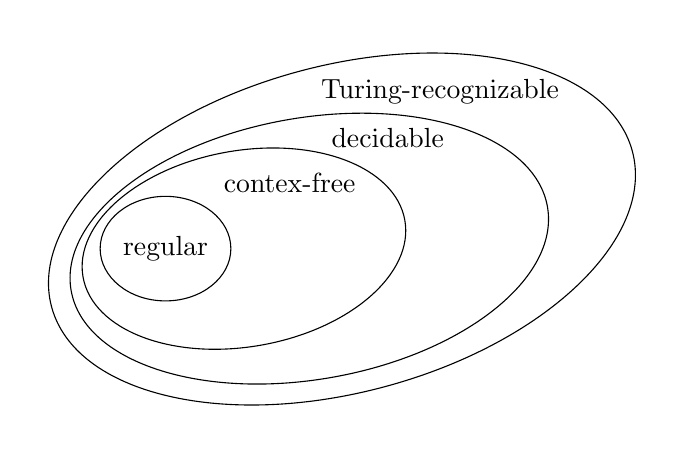
\begin{tikzpicture}[scale=0.83]
        % \draw (1,0) circle [radius=1.5];
        \draw (-3,0.3) circle [x radius=4.6cm, y radius=2.5cm, rotate=15];
        \draw (-3.5,0) circle [x radius=3.7cm, y radius=2cm, rotate=10];
        \draw (-4.5,0) circle [x radius=2.5cm, y radius=1.5cm, rotate=10];
        \draw (-5.7,0) circle [x radius=1cm, y radius=0.8cm];
        \path (-5.7,0) node {regular};
        \path (-3.8,1) node {contex-free};
        \path (-2.3,1.7) node {decidable};
        \path (-1.5,2.4) node {Turing-recognizable};  
    \end{tikzpicture}
    \caption{Classes of Languages}
\end{figure}

\newpage

\section{Halting Problem}

In program verification is in general undecidable (unsolvable). Here is a classic example of undecidable problem, the \textbf{Halting Problem}.

\subsection{Diagonalization Method}

\begin{definition}
    Two set are equal if elements can be paired up.
\end{definition}

Giving an example 

\begin{definition}[one-to-one function]
    A fucntion $f: A \to B$ is one-to-one if \[
        f(a) \neq f(b) \text{ if } a \neq b
    \]
\end{definition}

\begin{definition}[onto function]
    A function $f: A \to B$ is onto if \[
        \forall b \in B,\ \exists a \in A \text{ such that } f(a) = b
    \]
\end{definition}

\begin{definition}[correspondence]
    A \textbf{correspondence} between two sets $A$ and $B$ is a function $f: A \to B$ that is both one-to-one and onto.
\end{definition}

\begin{eg}
    Consider the function
    \begin{equation*}
    f(a) = a^2, \text{ where } A = (-\infty, \infty) \text{ and }
    B = (-\infty, \infty)
    \end{equation*}
\end{eg}
This is not an onto function because for $b = -1$, there is no $a \in A$ such that $f(a) = b$.

\begin{eg}
    Consider the function
    \begin{equation*}
    f(a) = a^2, \text{ where } A = [0, \infty) \text{ and }
    B = [0, \infty)
    \end{equation*}
\end{eg}
Becoming an onto function. However, it is not one-to-one because $f(1) = f(-1) = 1$.

\begin{eg}
    Consider the function
    \begin{equation*}
    f(a) = a^3, \text{ where } A = (-\infty, \infty) \text{ and }
    B = (-\infty, \infty)
    \end{equation*}
\end{eg}
This is a correspondence because it is both one-to-one and onto.
\begin{remark}
    Correspondence is a way to pair the elements in two sets. If there is a correspondence between two sets, then they have the same cardinality (size).
\end{remark}

\begin{definition}[countable]
    A set $A$ is \textbf{countable} if there is a correspondence between $A$ and $\mathbb{N}$ or a finite subset of $\mathbb{N}$.
\end{definition}

\newpage

\begin{theorem}
    Consider the set of rational numbers $\mathbb{Q}$, where \[
        \mathbb{Q} = \left\{ \frac{m}{n} \;\middle|\; m,n \in \mathbb{N} \right\}
    \]
    which is countable.
\end{theorem}
\vspace{-1em}
\begin{proof}
    Here is one way to list all the rational numbers:
    \begin{figure}[H]
        \centering
        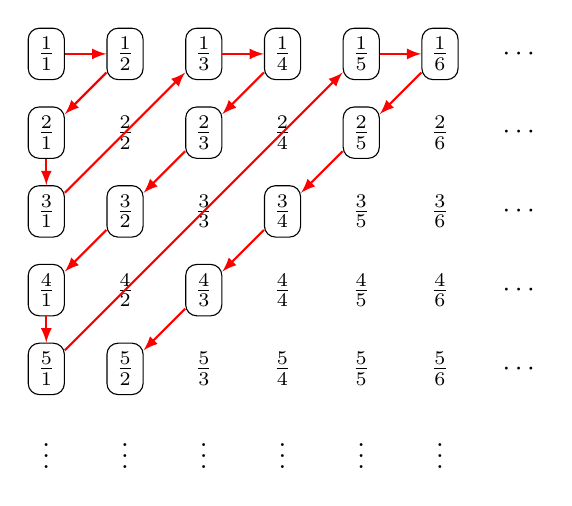
\begin{tikzpicture}
        \tikzstyle{keepstyle} =[rectangle, rounded corners, draw, fill=white]
        \node at (0,0) {$\vdots$};
        \node[keepstyle] (51) at (0,1) {$\frac{5}{1}$};
        \node[keepstyle] (41) at (0,2) {$\frac{4}{1}$};
        \node[keepstyle] (31) at (0,3) {$\frac{3}{1}$};
        \node[keepstyle] (21) at (0,4) {$\frac{2}{1}$};
        \node[keepstyle] (11) at (0,5) {$\frac{1}{1}$};
        \node at (1,0) {$\vdots$};
        \node[keepstyle] (52) at (1,1) {$\frac{5}{2}$};
        \node at (1,2) {$\frac{4}{2}$};
        \node[keepstyle] (32) at (1,3) {$\frac{3}{2}$};
        \node at (1,4) {$\frac{2}{2}$};
        \node[keepstyle] (12) at (1,5) {$\frac{1}{2}$};
        \node at (2,0) {$\vdots$};
        \node at (2,1) {$\frac{5}{3}$};
        \node[keepstyle] (43) at (2,2) {$\frac{4}{3}$};
        \node at (2,3) {$\frac{3}{3}$};
        \node[keepstyle] (23) at (2,4) {$\frac{2}{3}$};
        \node[keepstyle] (13) at (2,5) {$\frac{1}{3}$};
        \node at (3,0) {$\vdots$};
        \node at (3,1) {$\frac{5}{4}$};
        \node at (3,2) {$\frac{4}{4}$};
        \node[keepstyle] (34) at (3,3) {$\frac{3}{4}$};
        \node at (3,4) {$\frac{2}{4}$};
        \node[keepstyle] (14) at (3,5) {$\frac{1}{4}$};
        \node at (4,0) {$\vdots$};
        \node  at (4,1) {$\frac{5}{5}$};
        \node at (4,2) {$\frac{4}{5}$};
        \node at (4,3) {$\frac{3}{5}$};
        \node[keepstyle] (25) at (4,4) {$\frac{2}{5}$};
        \node[keepstyle] (15) at (4,5) {$\frac{1}{5}$};
        \node at (5,0) {$\vdots$};
        \node  at (5,1) {$\frac{5}{6}$};
        \node at (5,2) {$\frac{4}{6}$};
        \node at (5,3) {$\frac{3}{6}$};
        \node at (5,4) {$\frac{2}{6}$};
        \node[keepstyle] (16) at (5,5) {$\frac{1}{6}$};
        \node at (6,1) {$\cdots$};
        \node at (6,2) {$\cdots$};
        \node at (6,3) {$\cdots$};
        \node at (6,4) {$\cdots$};
        \node at (6,5) {$\cdots$};
        \draw [-latex,red, thick] (11) -- (12);
        \draw [-latex, red, thick] (12) -- (21);
        \draw [-latex, red, thick] (21) -- (31);
        \draw [-latex, red, thick] (31) -- (13);
        \draw [-latex, red, thick] (13) -- (14);
        \draw [-latex, red, thick] (14) -- (23);
        \draw [-latex, red, thick] (23) -- (32);
        \draw [-latex, red, thick] (32) -- (41);
        \draw [-latex, red, thick] (41) -- (51);
        \draw [-latex, red, thick] (51) -- (15);
        \draw [-latex, red, thick] (15) -- (16);
        \draw [-latex, red, thick] (16) -- (25);
        \draw [-latex, red, thick] (25) -- (34);
        \draw [-latex, red, thick] (34) -- (43);
        \draw [-latex, red, thick] (43) -- (52);
        \end{tikzpicture}
        \caption{Counting the rational numbers}
    \end{figure}
    
    However, for the set of real numbers $\mathbb{R}$, it is uncountable. We can use the diagonalization method to prove it.
\end{proof}

\begin{theorem}
    Consider the set of real numbers $\mathbb{R}$, which is uncountable.
\end{theorem}
\vspace{-1em}
\begin{proof}
    Assume $\mathbb{R}$ is countable, then we can list all the real numbers, we can construct a table of the corresponing decimal as follow:
    \begin{figure}[H]
        \centering
        \begin{tabular}{c|c}
            Index & Real Number \\
            \hline
            $1$ & $0.d_{11} d_{12} d_{13} d_{14} d_{15} \ldots$ \\
            $2$ & $0.d_{21} d_{22} d_{23} d_{24} d_{25} \ldots$ \\
            $3$ & $0.d_{31} d_{32} d_{33} d_{34} d_{35} \ldots$ \\
            $4$ & $0.d_{41} d_{42} d_{43} d_{44} d_{45} \ldots$ \\
            $5$ & $0.d_{51} d_{52} d_{53} d_{54} d_{55} \ldots$ \\
            $\vdots$ & $\vdots$
        \end{tabular}
        \caption{Listing all the real numbers}
    \end{figure}
    
    Then we consider a new real number $r = 0.r_1 r_2 r_3 \ldots$ where \[
        r_i = \begin{cases}
            5 & \text{if the } i\text{-th digit of } f(i) \neq 5\\
            6 & \text{if the } i\text{-th digit of } f(i) = 5
        \end{cases}
    \]
    By construction, \[
        r \neq f(n), \ \forall n \in \mathbb{N}
    \]
    But $r \in \mathbb{R}$, which contradicts our assumption. Therefore, $\mathbb{R}$ is uncountable.
\end{proof}

\begin{remark}
    To avoid \[
        1 = 0.999999\ldots
    \]
    we can simply avoid using $0, 9$ in our construction.
\end{remark}

\subsection{NOT Turing-Recognizable}

We known that $\Sigma^*$ is countable, because we can list all the strings in order of length. Also, the set of all \textbf{TMs is countable}, because each TM can be encoded as a string (i.e. set of TMs is a subset of $\Sigma^*$). \\

Now, let \[
    \begin{cases}
        L: \text{ set of all languages over } \Sigma \\
        B: \text{ set of all infinite binary sequences}
    \end{cases}
\]
For any language $A \subseteq \Sigma^*$, we can construct a corresponding infinite binary sequence $\chi_A = b_1 b_2 b_3 \ldots$ where \[
    b_i = \begin{cases}
        1 & \text{if } s_i \in A \\
        0 & \text{if } s_i \notin A
    \end{cases}
\]
where $s_1, s_2, s_3, \ldots$ is the enumeration of all strings in $\Sigma^*$. This construction is in diagonalization way. This gives a correspondence between $L$ and $B$. Since $B$ is uncountable (by diagonalization method), \textbf{$L$ is also uncountable}. \\

Each Turing machine corresponds to a language that it recognizes. Since the set of all TMs is countable, the set of all Turing-recognizable languages is also countable. Therefore, there are languages that are not Turing-recognizable.

\subsection{Halting Problem is Undecidable}

Racall that halting problem is defined as 

\begin{theorem}
    We define the language \[
        A_{\text{TM}} = \{ \langle M, w \rangle \mid M: \text{ TM that  accept } w \}
    \]
    The language $A_{\text{TM}}$ is undecidable.
\end{theorem}
\vspace{-1em}
\begin{proof}
    Assume $H$ is a TM that decides $A_{\text{TM}}$. Then we get \[
        H(\langle M, w \rangle) = \begin{cases}
            \text{accept} & \text{if } M \text{ accepts } w \\
            \text{reject} & \text{Otherwise}
        \end{cases}
    \]
    Then we can construct a new TM $D$ with $H$ by running it on input $\langle M, \langle M \rangle \rangle$. The behavior of $D$ is defined as follows:
    \[
        D(\langle M \rangle) = \begin{cases}
            \text{accept} & \text{if } H(\langle M, \langle M \rangle \rangle) = \text{reject} \\
            \text{reject} & \text{if } H(\langle M, \langle M \rangle \rangle) = \text{accept}
        \end{cases}
    \]
    which can be simplified as \[
        D(\langle M \rangle) = \begin{cases}
            \text{accept} & \text{if } M \text{ rejects } \langle M \rangle \\
            \text{reject} & \text{if } M \text{ accepts } \langle M \rangle
        \end{cases}
    \]
    But we have a contradiction when we run $D$ on input $\langle D \rangle$:
    \[
        D(\langle D \rangle) = \begin{cases}
            \text{accept} & \text{if } D \text{ rejects } \langle D \rangle \\
            \text{reject} & \text{if } D \text{ accepts } \langle D \rangle
        \end{cases}
    \]
\end{proof}

\begin{note}
    The diagonalization method is use in here again. Set of TMs is countable, so we can list all the TMs as $M_1, M_2, M_3, \ldots$. Then we can construct a table as follows:
    \begin{figure}[H]
        \centering
        \begin{tabular}{c|cccc}
            & $M_1$ & $M_2$ & $M_3$ & $\cdots$ \\
            \hline
            $\langle M_1 \rangle$ & $b_{11}$ & $b_{12}$ & $b_{13}$ & $\cdots$ \\
            $\langle M_2 \rangle$ & $b_{21}$ & $b_{22}$ & $b_{23}$ & $\cdots$ \\
            $\langle M_3 \rangle$ & $b_{31}$ & $b_{32}$ & $b_{33}$ & $\cdots$ \\
            $\vdots$ & $\vdots$ & $\vdots$ & $\vdots$ & $\ddots$
        \end{tabular}
        \caption{Listing all the TMs and their behavior on their own encoding}
    \end{figure}
    where \[
        b_{ij} = \begin{cases}
            1 & \text{if } M_j \text{ accepts } \langle M_i \rangle \\
            0 & \text{if } M_j \text{ rejects, or loops on } \langle M_i \rangle
        \end{cases}
    \]
    Then we know $H$ decides $A_{\text{TM}}$ as it is a decider, we have 
    \begin{figure}[H]
        \centering
        \begin{tabular}{c|cccc}
            & $M_1$ & $M_2$ & $M_3$ & $\cdots$ \\
            \hline
            $\langle M_1 \rangle$ & $b_{11}$ & $b_{12}$ & $b_{13}$ & $\cdots$ \\
            $\langle M_2 \rangle$ & $b_{21}$ & $b_{22}$ & $b_{23}$ & $\cdots$ \\
            $\langle M_3 \rangle$ & $b_{31}$ & $b_{32}$ & $b_{33}$ & $\cdots$ \\
            $\vdots$ & $\vdots$ & $\vdots$ & $\vdots$ & $\ddots$
        \end{tabular}
        \caption{Listing all the TMs and their behavior on their own encoding}
    \end{figure}
    where \[
        b_{ii} = \begin{cases}
            A & \text{if } M_i \text{ accepts } \langle M_i \rangle \\
            R & \text{if } M_i \text{ rejects } \langle M_i \rangle
        \end{cases}
    \]
    Then we can construct a new TM $D$ which output the opposite of the diagonal entries, then we get a contradiction when we run $D$ on input $\langle D \rangle$.
    \begin{figure}[H]
        \centering
        \begin{tabular}{c|cccc}
            & $\langle  M_1\rangle $ & $\langle  M_2\rangle $ & $\ldots$ & $\langle  D\rangle $\\ \hline
            $M_1$ & R & &&\\
            $M_2$ &  & R && \\
            && & $\ddots$ & \\
            $D$ &&&& \red{\textbf{?}}
        \end{tabular}
    \caption{Contradiction on the diagonal entries}
    \end{figure}
\end{note}

\newpage

\subsection{co-Turing-Recognizable}

\begin{definition}[co-Turing-recognizable]
    A language $L$ is \textbf{co-Turing-recognizable} if its complement $\overline{L}$ is Turing-recognizable.
\end{definition}

\begin{theorem}
    A language $L$ is decidable if and only if it is both Turing-recognizable and co-Turing-recognizable.
\end{theorem}
\vspace{-1em}
\begin{proof}
    We seperately prove the two directions.
    \begin{itemize}
        \item[$\Rightarrow$] If $L$ is decidable, then there is a TM $M$ that decides $L$. We can use $M$ to recognize $L$ and $\overline{L}$. Hence, $L$ is both Turing-recognizable and co-Turing-recognizable.
        \item[$\Leftarrow$] Now $A, \overline{A}$ are both Turing-recognizable by TM $M_1$ and $M_2$ respectively. We can construct a new TM $M$ that decides $L$ as follows:
        \begin{enumerate}[label=$\arabic*^\circ$]
            \item On input $w$, run $M_1$ and $M_2$ in parallel on input $w$.
            \item If $M_1$ accepts, then accept. If $M_2$ accepts, then reject.
        \end{enumerate}
        Since $w \in L$ or $w \notin L$, either $M_1$ or $M_2$ will eventually accept $w$. Thus, $M$ halts on all inputs, and decides $L$.
    \end{itemize}
    Proof complete.
\end{proof}